\documentclass[11pt]{article}
\usepackage{amsmath, amssymb}
\usepackage{geometry}
\geometry{margin=1in}
\usepackage{fancyhdr}
\usepackage{lastpage}
\usepackage{parskip} % Better paragraph spacing
\usepackage{titlesec} % Better section formatting
\usepackage{graphicx}
\usepackage{float}
\usepackage[most]{tcolorbox}
\usepackage{lmodern}
\usepackage{caption}
\usepackage{hyperref}
\usepackage{listings}
\usepackage{xcolor}

\definecolor{codegreen}{rgb}{0,0.6,0}
\definecolor{codegray}{rgb}{0.5,0.5,0.5}
\definecolor{codepurple}{rgb}{0.58,0,0.82}
\definecolor{backcolour}{rgb}{0.95,0.95,0.92}

% Define code styling
\lstdefinestyle{mystyle}{
    backgroundcolor=\color{backcolour},
    commentstyle=\color{codegreen},
    keywordstyle=\color{magenta},
    numberstyle=\tiny\color{codegray},
    stringstyle=\color{codepurple},
    basicstyle=\ttfamily\footnotesize,
    breakatwhitespace=false,
    breaklines=true,
    captionpos=b,
    keepspaces=true,
    numbers=left,
    numbersep=5pt,
    showspaces=false,
    showstringspaces=false,
    showtabs=false,
    tabsize=2
}

\lstset{style=mystyle}

% Define commands for reusable content
\newcommand{\coursename}{CS-401 Applied Data Analysis}
\newcommand{\lecturenum}{08}
\newcommand{\lecturedate}{05/11/2025}
\newcommand{\professor}{Maria Brbic}

\hypersetup{colorlinks=true,linkcolor=blue,urlcolor=blue}

% Configure section spacing
\titlespacing*{\section}{0pt}{2ex plus 1ex minus .2ex}{1.5ex plus .2ex}
\titlespacing*{\subsection}{0pt}{1.5ex plus 1ex minus .2ex}{1ex plus .2ex}
% Header / Footer
\pagestyle{fancy}
\fancyhf{}
\fancyhead[L]{\coursename}
\fancyhead[R]{Lecture \lecturenum}
\fancyfoot[L]{EPFL - Computer Science}
\fancyfoot[C]{Author: Jonathan Dutoit}
\fancyfoot[R]{Page \thepage\ of \pageref{LastPage}}

\begin{document}

\begin{center}
  {\large EPFL - Computer Science} \\[0.5em]
  {\Large \textbf{\coursename}} \\[0.5em]
  {\large Lecture \lecturenum\ --- \lecturedate} \\[0.5em]
  {\large Author: Jonathan Dutoit} \\[0.5em]
  {\large Professor: \professor} \\[0.5em]
\end{center}

\vspace{2cm}

\begin{center}
  {\LARGE \textbf{Applied Machine Learning}}
\end{center}

\vspace{1cm}
\section*{Classification pipeline}

$\oplus \Rightarrow$ Data collection $\Rightarrow$ Model Selection $\Rightarrow$ Model assessment $\Rightarrow \oplus$

\section*{Data collection}

The first step is collecting data related to the classification task.
\begin{itemize}
	\item Definition of the attributes (or features) that describe a data item and the class label.
\end{itemize}

Domain knowledge is needed. 

What if assigning the class label would be too time-consuming or even impossible?
\begin{itemize}
	\item \textcolor{green}{Unsupervised methods} (e.g., clustering)
\end{itemize}

% Quick centered image
\begin{figure}[H]
    \centering
    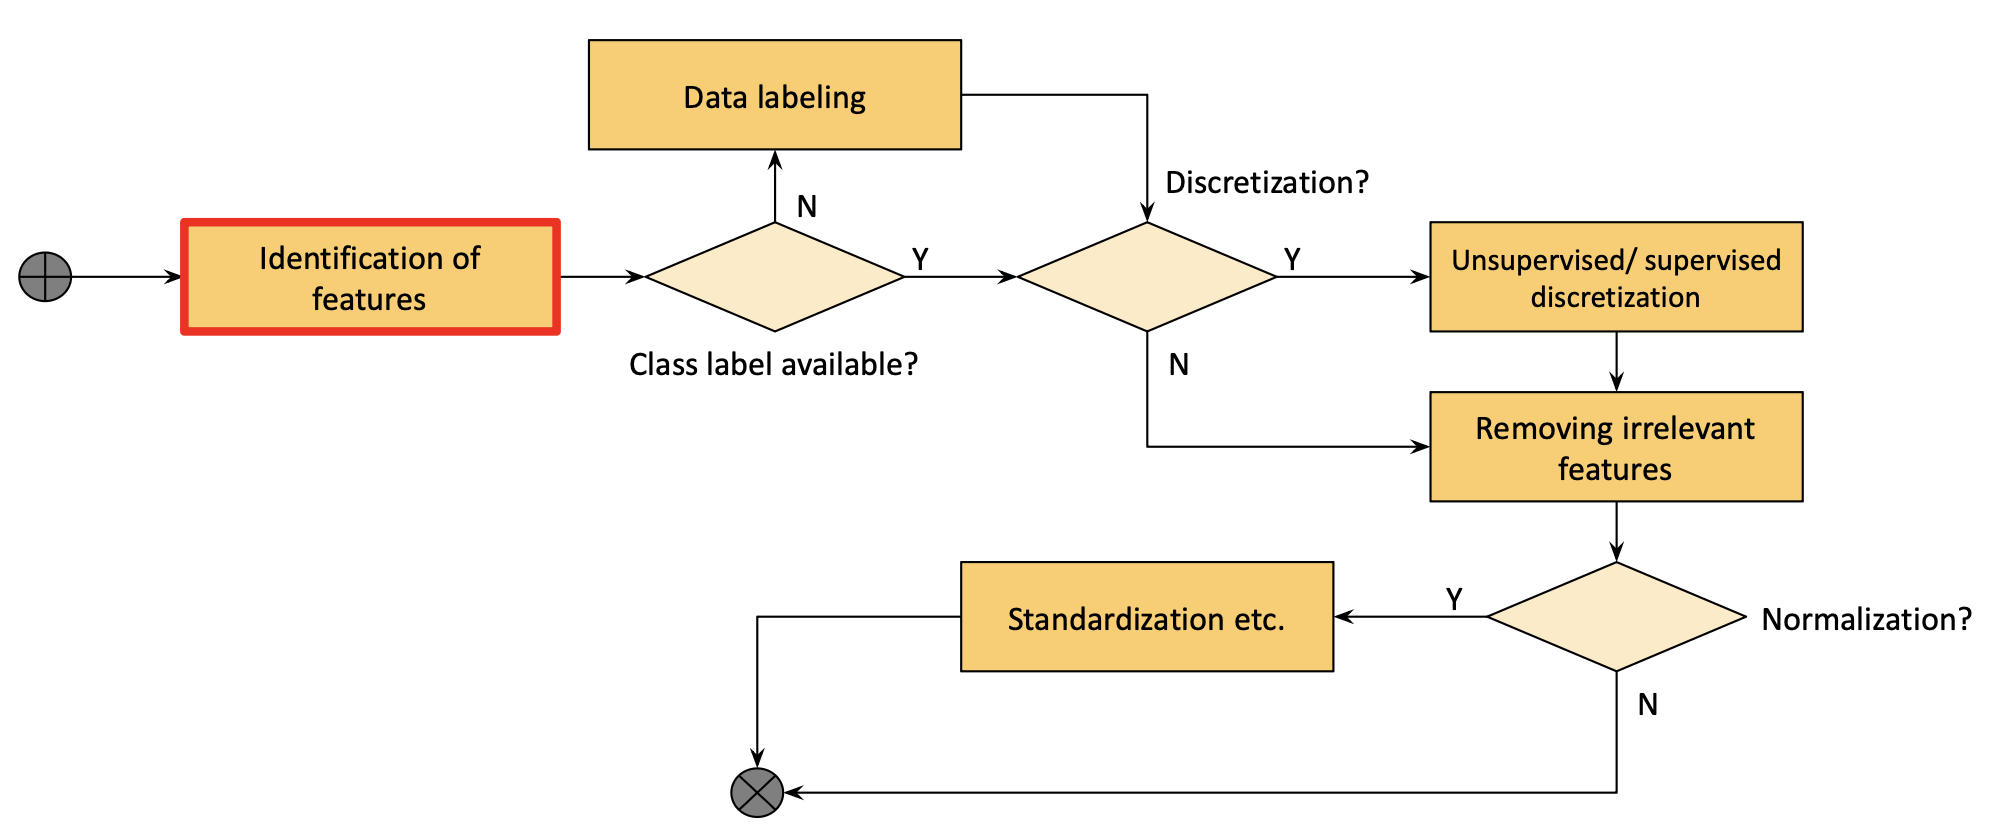
\includegraphics[width=0.8\textwidth]{data-collection}
    \label{fig:LABEL}
\end{figure}

\subsection*{Features}

Different types of features
\begin{itemize}
	\item Continuous (e.g., height, temperature, ...)
	\item Ordinal (e.g., "agree", "don't care", "disagree", ...)
	\item Categorical (e.g., country, gender, ...)
\end{itemize}

New features can be generated from \textcolor{green}{simple stats}
\begin{itemize}
	\item \textcolor{blue}{\textbf{\textit{Feature engineering}}} is considered a form of art, therefore it is often useful to find what other people did for similar problems
\end{itemize}

Some classifiers require categorical features $\Rightarrow$ \textcolor{purple}{discretization}

\subsection*{Labels}

Collecting a lot of data (features) is often easy. Labeling data is time consuming, difficult, and sometimes even possible. Often \textit{human expertise} is needed. 

\subsection*{Potential labelers}
\begin{itemize}
	\item You
	\item Older days:
		\begin{itemize}
			\item Undergraduate students
			\item Domain experts (\$\$\$)
		\end{itemize}
	\item Now: \textcolor{green}{crowdsourcing}
		\begin{itemize}
			\item Can get both amateurs ($\sim$ undergrad students) and experts
		\end{itemize}
\end{itemize}

% Quick centered image
\begin{figure}[H]
    \centering
    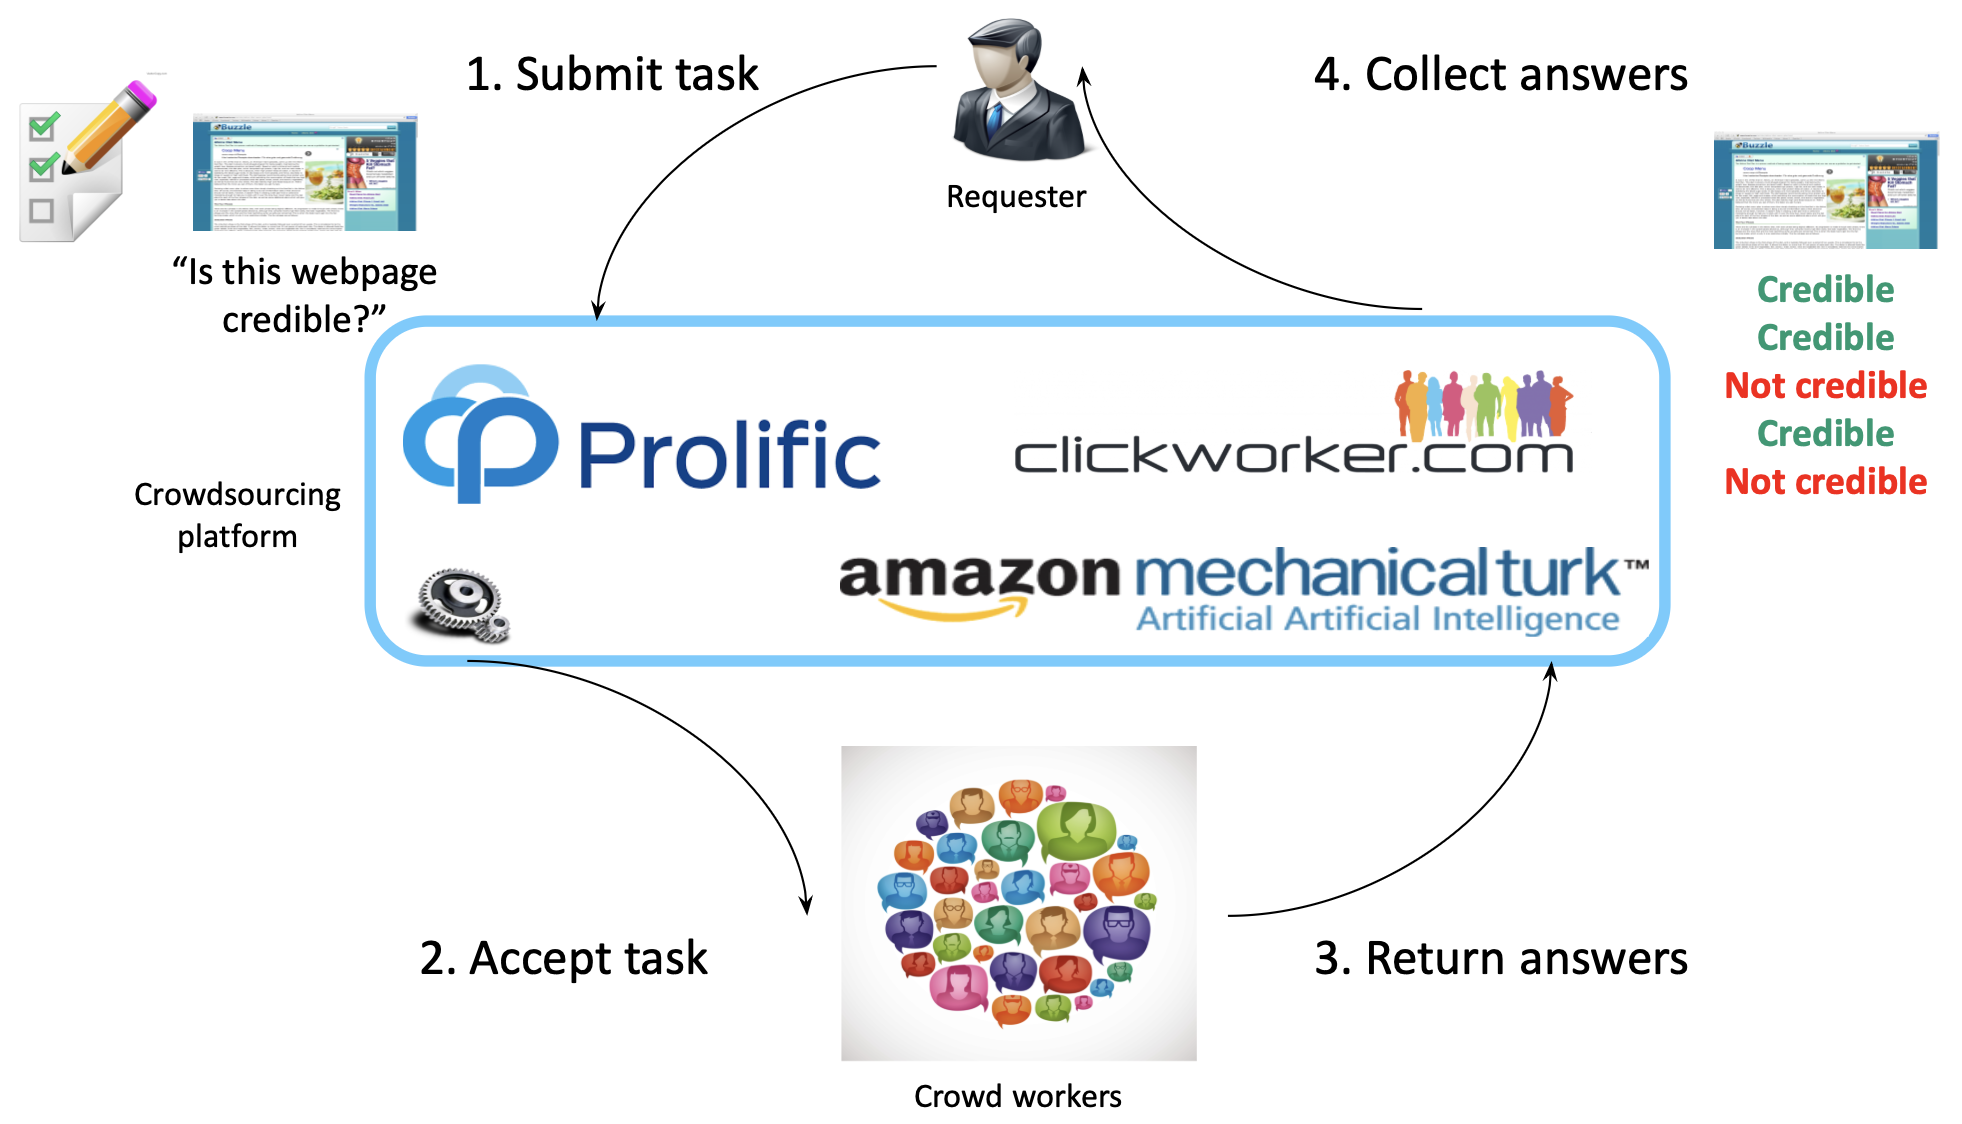
\includegraphics[width=0.8\textwidth]{crowd-sourcing}
    \label{fig:LABEL}
\end{figure}

\subsection*{Discretization}

\textbf{Why?}
\begin{itemize}
	\item Some classifiers want discrete features (e.g., simplets kinds of decision trees)
	\item Discrete features let a linear classifier learn non-linear decision boundaries
	\item Certain features selection methods require discrete (or even binary) features
\end{itemize}

\newpage
\textbf{\textcolor{blue}{Unsupervised}}: we don't want to use class labels for discretization
\begin{itemize}
	\item \textcolor{red}{Equal width}
		\begin{itemize}
			\item Divide the range into a predefined number of bins (bad for skewed data, e.g., from a power law)
		\end{itemize}
	\item \textcolor{red}{Equal frequency}
		\begin{itemize}
			\item Divide the range into a predefined number of bins so that every interval contains the same number of values. Doesn't take into account natural grouping of features.
		\end{itemize}
	\item \textcolor{red}{Clustering}
\end{itemize}

\textbf{\textcolor{blue}{Supervised}}: we use the class labels in order to perform discretization
\begin{itemize}
	\item Start with very fine-grained discretization
	\item Test the hypothesis that membership in two adjacent intervals of a feature is independent of the class
	\item If they are independent, they should be merge
	\item Otherwise they should remain separate 
	\item Independence test: $\chi^{2}$ test ("chi-squared test")
	\item Continue recursively
\end{itemize}

\subsection*{Removing irrelevant features: Feature selection}

\begin{itemize}
	\item \textcolor{purple}{\textbf{Goal}}: reduce set of \textit{N} features to a subset of the best size \textit{M} $<$ \textit{N}
	\item \textbf{\textcolor{blue}{Why?}}
		\begin{itemize}
			\item More interpretability
	\item Less danger of overfitting
	\item More efficient training
\end{itemize}
	\item \textbf{\textcolor{red}{Problem}}: There are $2^{N}$ possible subsets
	\item \textbf{\textcolor{green}{Solutions}}
		\begin{itemize}
			\item Filtering as preprocessing ("offline")
	\item Iterative feature selection ("online")
\end{itemize}
\end{itemize}

\textbf{\textcolor{red}{Offline feature selection}}

Rank features according to their individual predictive power; then select the best ones

\begin{itemize}
	\item \textbf{\textcolor{green}{Pros}}
		\begin{itemize}
			\item Independent of the classifiers (performed only once)
		\end{itemize}
	\item \textbf{\textcolor{red}{Cons}}
		\begin{itemize}
			\item Independent of the classifiers (ignore interaction with the classifier)
			\item Assumes features are independent
		\end{itemize}
\end{itemize}

\textbf{\textcolor{red}{Ranking of features}}

\textbf{\textcolor{purple}{Continuous features (and ideally labels):}}
\begin{itemize}
	\item Pearson's correlation coefficient (capturing strength of linear [!] dependence)
		\[
			r = \frac{\sum_{i=1}^{n}(X_i - \bar{X})(Y_i - \bar{Y})}{\sqrt{\sum_{i=1}^{n}(X_i - \bar{X})^{2}} \sqrt{\sum_{i=1}^{n}(Y_i - \bar{Y})^{2}}} 
		.\] 
\end{itemize}

\textbf{\textcolor{blue}{Categorical features and labels:}}
\begin{itemize}
	\item Mutual information (goes beyond linear dependence)
		\begin{center}
			\textit{I(F;C) = H(C) - H(C $\mid$ F) = H(F) + H(C) - H(F, C)} \\
			\textit{H(F) =} -$\underset{i}{\sum} P(f_i) \log_2 P(f_i)$ \\
			\textit{H(F, C) =} $- \underset{i}{\sum} \underset{j}{\sum} P(f_i, c_j) \log_2 P(f_i, c_j)$ 
		\end{center}
	\item $\chi^{2}$ method ("chi-squared") 
		\begin{itemize}
			\item Similar to $\chi^{2}$ method for feature discretization
	\item Test whether the feature is independent of label
	\item Different w.r.t. mutual information: the $\chi^{2}$ test checks the independence of the class and the feature, without indicating the strength or direction of any existing relationship (you just get a significance, a.k.a \textit{p-value})
\end{itemize}
	\item \textbf{\textcolor{red}{Beware}}: collectively relevant features may look individually irrelevant!		
\end{itemize}


\textbf{\textcolor{red}{Online feature selection}}

\textbf{\textcolor{purple}{Forward feature selection}}: greedily \textcolor{orange}{add} features; evaluate on validation dataset; stop when no improvement. 

\begin{itemize}
	\item \textbf{\textcolor{green}{Pros}}
		\begin{itemize}
			\item Interact with the classifier
			\item No feature-independence assumption
		\end{itemize}
	\item \textbf{\textcolor{red}{Cons}}
		\begin{itemize}
			\item Computationally intensive
		\end{itemize}
\end{itemize}

\textbf{\textcolor{purple}{Backward feature selection}}: greedily \textcolor{orange}{remove} features; evaluate on validation dataset; stop when no improvement
\begin{itemize}
	\item \textbf{\textcolor{green}{Pros}}
		\begin{itemize}
			\item Interact with the classifier
			\item No feature-independence assumption
		\end{itemize}
	\item \textcolor{red}{\textbf{Cons}}
		\begin{itemize}
			\item Computationally intensive
		\end{itemize}
\end{itemize}

\newpage
\subsection*{Feature normalization}

\begin{itemize}
	\item Some classifiers can't easily handle features with different scales, e.g., 
		\begin{itemize}
			\item Revenue in CHF: 10,000,000
			\item # of employees: 300
		\end{itemize}
	\item Features with large values dominate the others, and the classifiers tends to over-optimize for them
	\item Even single feature may span many orders of magnitude
		\begin{itemize}
			\item e.g., city size (most cities small, some huge)
			\item Too little resolutions where data is dense, too much resolution where data is sparse
		\end{itemize}
\end{itemize}

\textbf{\textcolor{red}{Logarithmic scaling}}
\[
x_i^{'} = \log(x_i)
.\] 
\begin{itemize}
	\item Consider order of magnitude, rather than direct value
	\item Good for heavy-tailed features (e.g, from power laws)
\end{itemize}

\textcolor{red}{\textbf{Min-max scaling}}
\[
x_i^{'} = (x_i - m_i)/(M_i - m_i)
.\] 

where $M_i$ and $m_i$ are the max and min values of feature $x_i$ respectively. The new feature $x_i^{'}$ lies in the interval [0, 1]

\textcolor{red}{\textbf{Standardization}}
\[
x_i^{'} = (x_i - \mu_i)/\sigma_i
.\] 

where $\mu_i$ is the mean value of feature $x_i$, and $\sigma_i$ is the standard deviation. The new feature $x_i^{'}$ has mean 0 and standard deviation 1

\textcolor{red}{\textbf{Dangers of standardization and scaling}}

\textcolor{orange}{Standardization}
\begin{itemize}
	\item Assume that the data has been generated by Gaussian
	\item Users mean and std $\Rightarrow$ not meaningful for heavy-tailed data (may be mitigated by log-scaling)
\end{itemize}
\textcolor{green}{Min-max scaling}
\begin{itemize}
	\item If the data has outliers, they scale the typical values to a very small interval
\end{itemize}

\section*{Model selection}

\textcolor{red}{\textbf{Model selection: high level}}

\textbf{Need to choose type of model}
\begin{itemize}
	\item k-NN?
	\item Decision trees?
	\item random forest?
	\item Boosted decision trees?
	\item Logistic regression?
	\item Deep learning?
\end{itemize}

\textbf{\textcolor{red}{Model selection: low level}}

\textbf{Usually a classifier has some "\textcolor{green}{hyperparameters}" to be tuned}
\begin{itemize}
	\item Set of features to include
	\item Distance function (e.g., k-NN)
	\item Number of neighbors (e.g., k-NN)
	\item Number of trees (e.g., random forest)
	\item Decision threshold (e.g., logistic regression)
	\item Regularization parameter
	\item Learning rate (for gradient descent algorithms)
\end{itemize}

\textcolor{red}{\textbf{Loss function}}
\begin{itemize}
	\item Categorical output
		\begin{itemize}
			\item e.g., 0-1 loss function, risk (= 1 minus accuracy):
				\[
					J = \frac{1}{n} \sum_{i=1}^{n} \# (y \neq f(x_i))
				.\] 
		\end{itemize}
	\item Real-valued output
		\begin{itemize}
			\item e.g., squared error:
				\[
				J = \frac{1}{n} \sum_{i=1}^{n} (y_i - f(x_i))^{2}
				.\] 
			\item e.g., absolute error:
				\[
				J = \frac{1}{n} \sum_{i=1}^{n} \mid y_i - f(x_i)\mid
				.\] 
		\end{itemize}
\end{itemize}

\subsection*{On what data to evaluate?}

% Quick centered image
\begin{figure}[H]
    \centering
    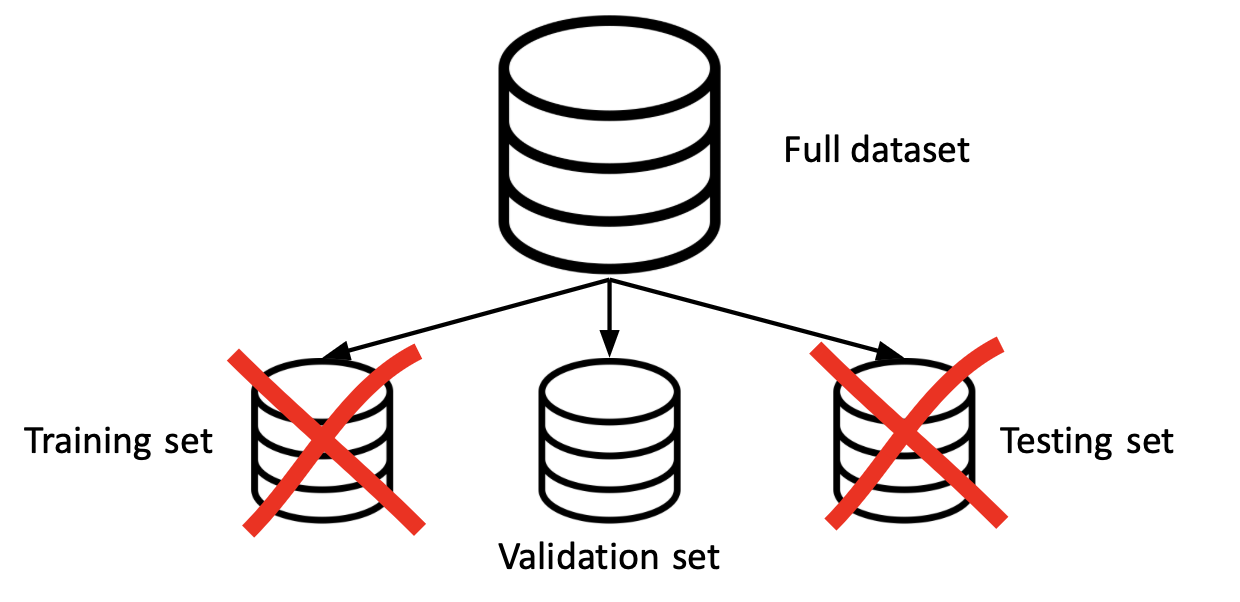
\includegraphics[width=0.65\textwidth]{dataset}
    \label{fig:LABEL}
\end{figure}

The validation set helps us to pick the right model! 

What if you can't afford a 3-way split because you have too little data?

$\Rightarrow$ \textcolor{blue}{\textbf{Cross-validation}}

\subsection*{Cross-validation}

% Quick centered image
\begin{figure}[H]
    \centering
    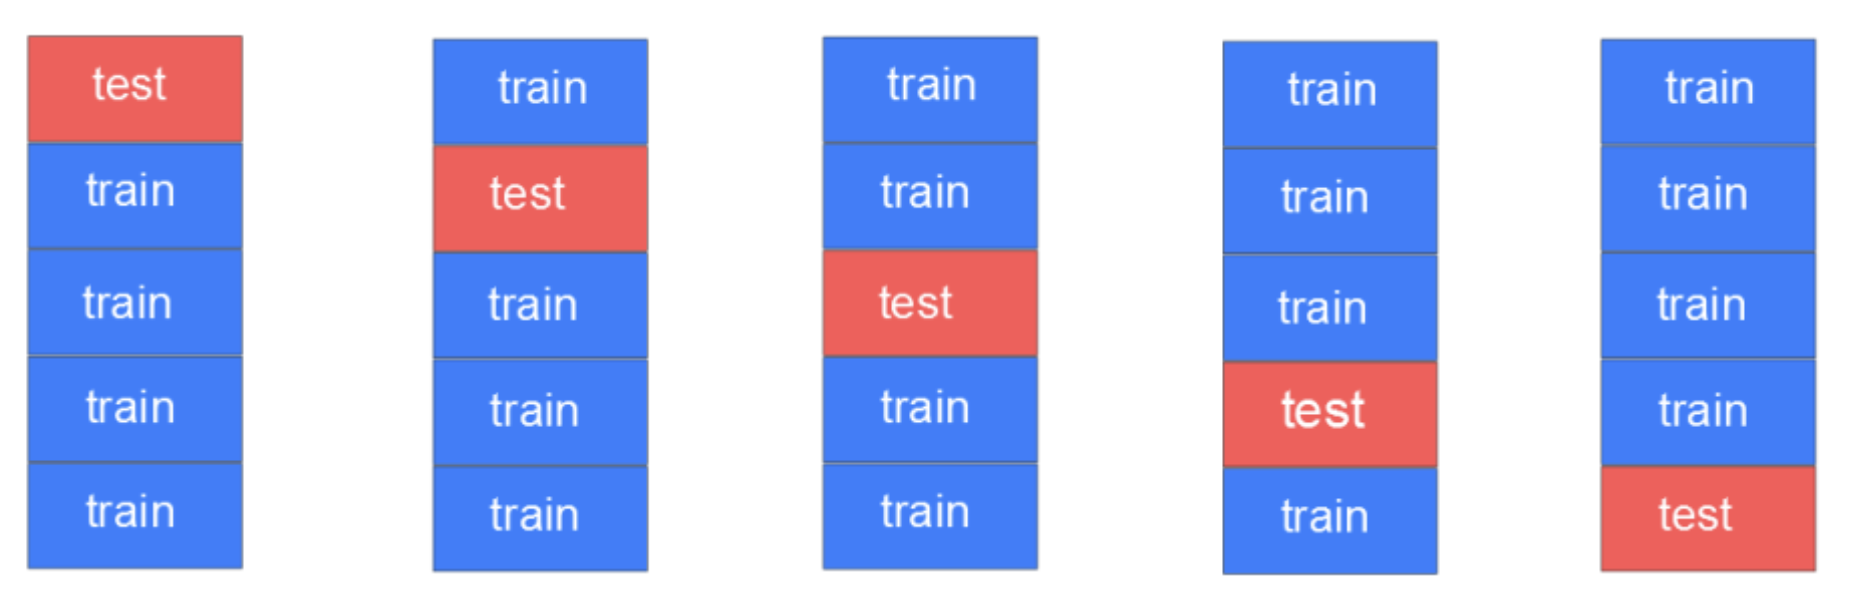
\includegraphics[width=0.8\textwidth]{cross-valid}
    \label{fig:LABEL}
\end{figure}

\begin{itemize}
	\item Last lecture: \textcolor{blue}{leave-one-out cross-validation} == N-fold cross-validation (where \textit{N} is the $\#$data points). This is quite computationally expensive. 
	\item More efficient: \textit{m}-fold cross-validation (in above picture: m=5)
	\item Average performance over the \textit{m} red portions $\Rightarrow$ validation error
	\item Repeat procedure for all candidate models and pick the one with the lowest validation error
\end{itemize}

Example: number of neighbors in k-NN
% Quick centered image
\begin{figure}[H]
    \centering
    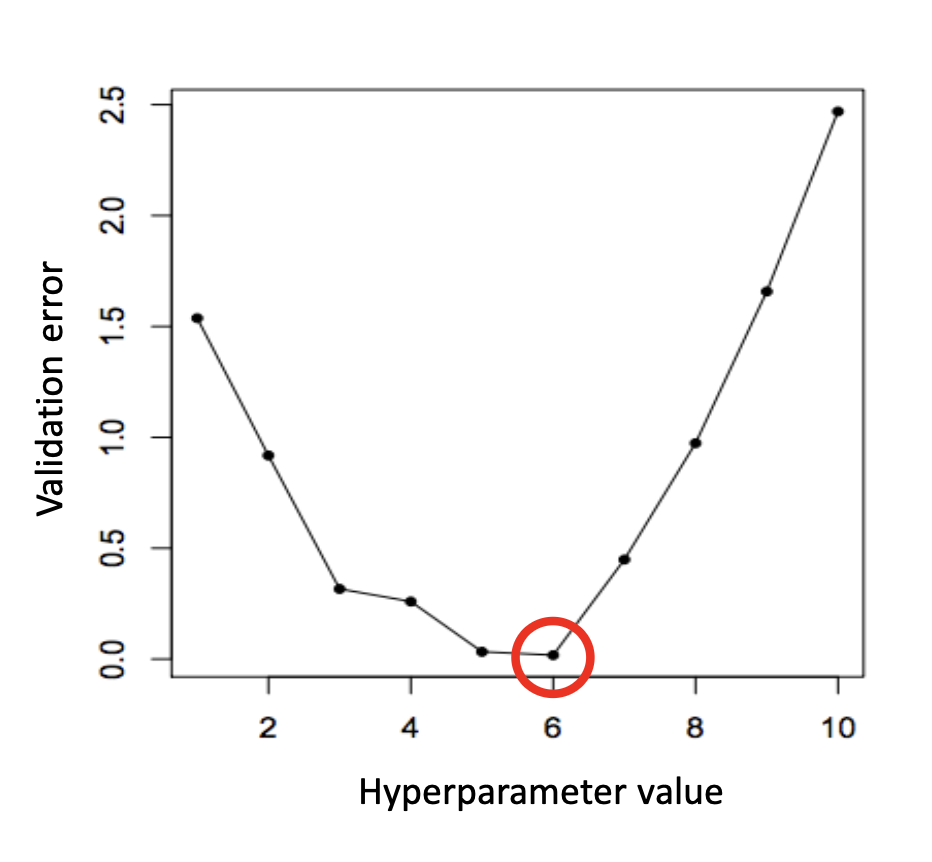
\includegraphics[width=0.5\textwidth]{valid-error}
    \label{fig:LABEL}
\end{figure}


\subsection*{Performance metrics for binary classification}

For categorical binary classification, the usual metrics are based on the \textcolor{blue}{confusion matrix}, which has 4 values:
\begin{itemize}
	\item True Positives (positive examples classified as positive)
	\item True Negatives (negative examples classified as negative)
	\item False positives (negative examples classified as positive)
	\item False Negatives (positive examples classified as negative)
\end{itemize}
% Quick centered image
\begin{figure}[H]
    \centering
    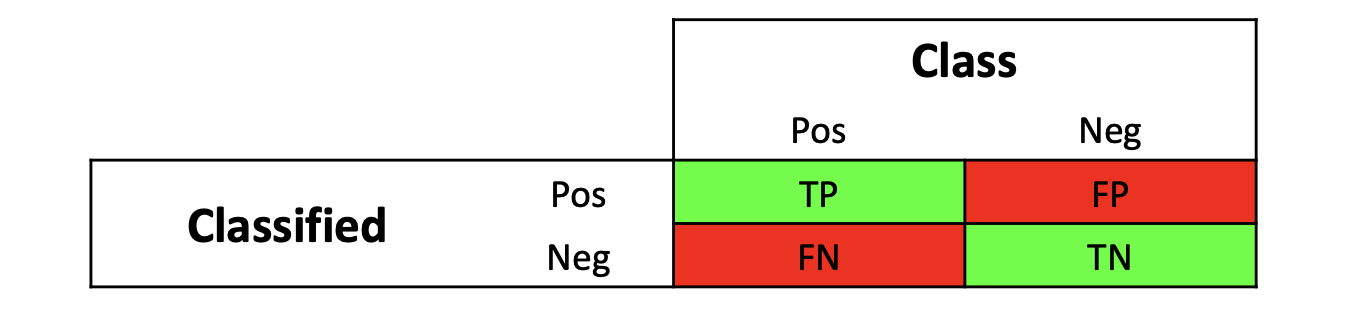
\includegraphics[width=0.65\textwidth]{confusion-matrix}
    \label{fig:LABEL}
\end{figure}


\subsection*{Accuracy}

\begin{center}
	\textit{A = }$\frac{TP + TN}{TP+TN+FP+FN}$ = $\frac{TP+TN}{N}$
\end{center}

Appropriate metric when
\begin{itemize}
	\item classes are not skewed
	\item errors (FP, FN) have the same importance
\end{itemize}

\subsection*{Accuracy (skewed example)}
% Quick centered image
\begin{figure}[H]
    \centering
    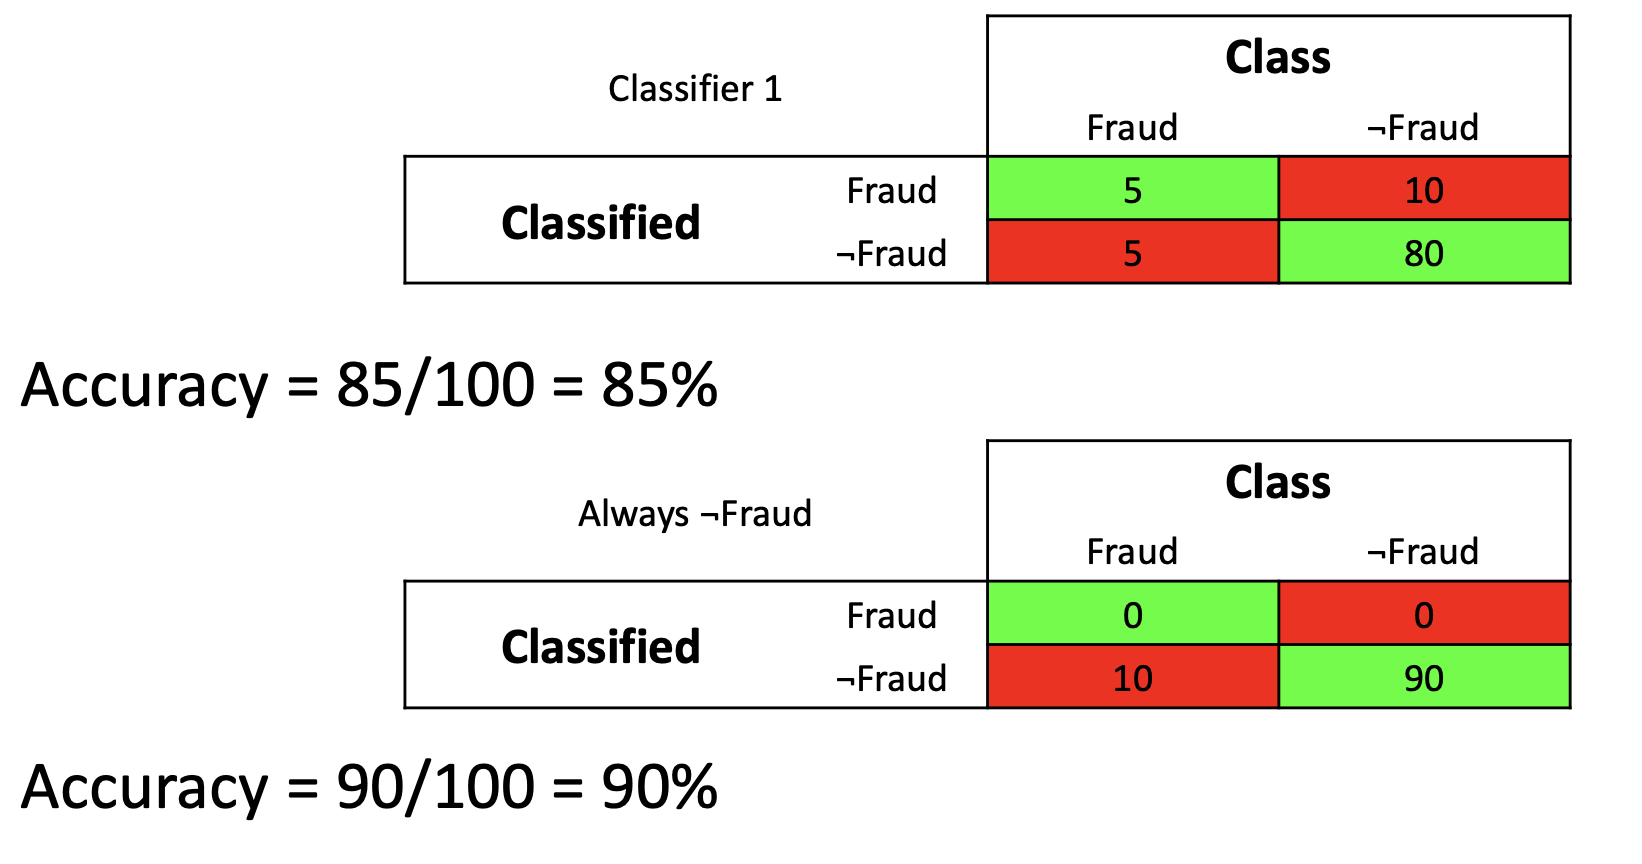
\includegraphics[width=0.65\textwidth]{accuracy-skewed}
    \label{fig:LABEL}
\end{figure}

The second classifier always says no but has higher accuracy...


\subsection*{Precision}

What fraction of positive predictions are actually positive?

\begin{center}
          P = $\frac{TP}{TP+FP}$
\end{center}

\subsection*{Recall}

What fraction of actually positive examples did I recognize as such?

\begin{center}
          R = $\frac{TP}{TP+FN}$
\end{center}


% Quick centered image
\begin{figure}[H]
    \centering
    \includegraphics[width=0.8\textwidth]{cancer}
    \label{fig:LABEL}
\end{figure}

\begin{minipage}{0.5\textwidth}
\begin{itemize}
	\item Accuracy: 0.75
	\item Precision: 0.69
	\item Recall: 0.9
\end{itemize}
\end{minipage}
\hfill
\begin{minipage}{0.5\textwidth}
\begin{itemize}
	\item Accuracy: 0.8
	\item Precision: 0.8
	\item Recall: 0.8
\end{itemize}
\end{minipage}


In this case, \textbf{Recall} is more important because we want to recognize those who truly have cancer! But we should always take into account the trade-off between Recall and Precision!


\subsection*{F-score}

Sometime it's necessary to have a single metric to compare classifiers. 

F-score (or F1-score): harmonic mean of precision and recall:

\begin{center}
	\textit{F1 = } $2 \cdot \frac{P \cdot R}{P + R}$
\end{center}

Precision and recall can be \textbf{differently weighted}, if one is more important than the other. 

\subsection*{Precision/Recall curve}

% Quick centered image
\begin{figure}[H]
    \centering
    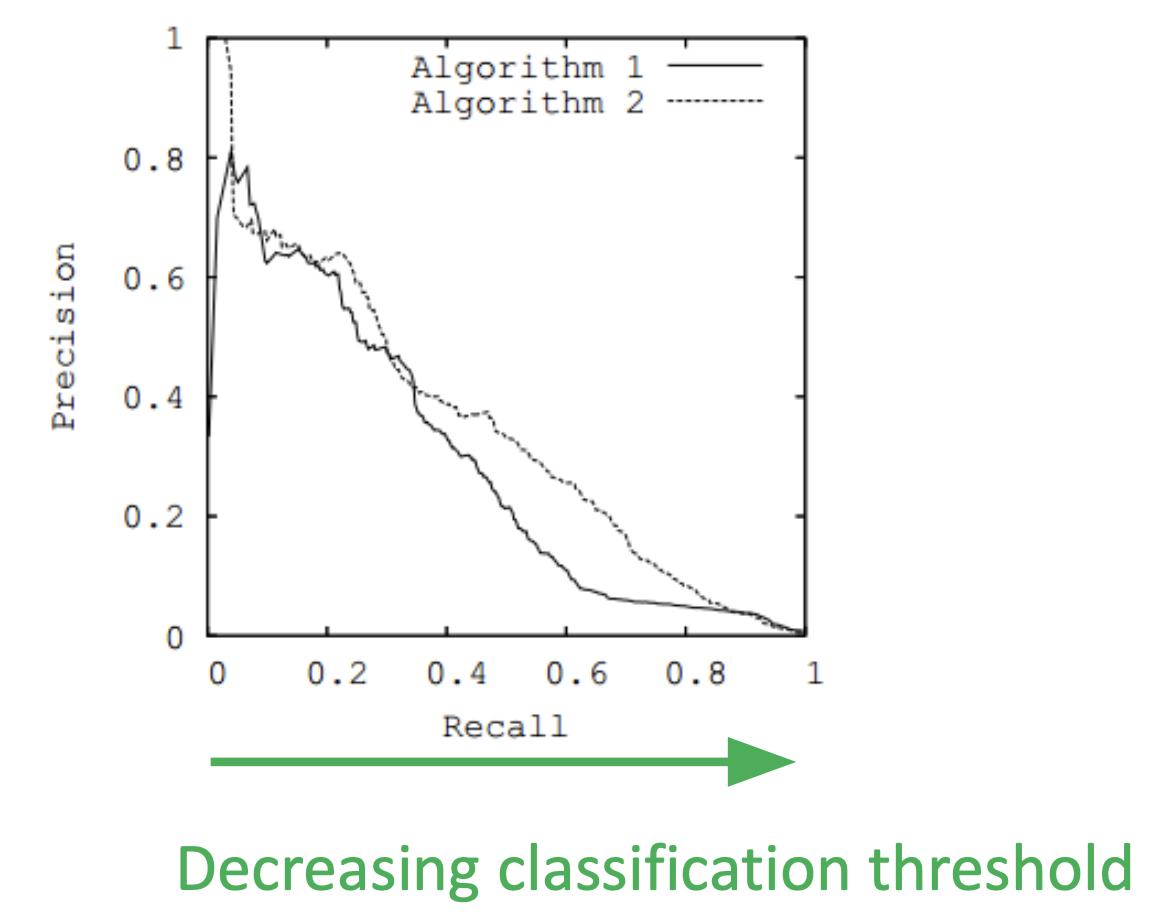
\includegraphics[width=0.6\textwidth]{pr-curve}
    \label{fig:LABEL}
\end{figure}

In this case we would chose algorithm 2 since it almost always a better performance. 

Precision/recall curve is very useful tool to compare models. There's no need to pre-select the decision threshold. 

\newpage

\subsection*{ROC curve}

ROC = Receive-Operating Characteristic

Y-axis: true-positive rate = TP/(TP + FN) a.k.a recall

X-axis: false-positve rate = FP/(FP + TN)

% Quick centered image
\begin{figure}[H]
    \centering
    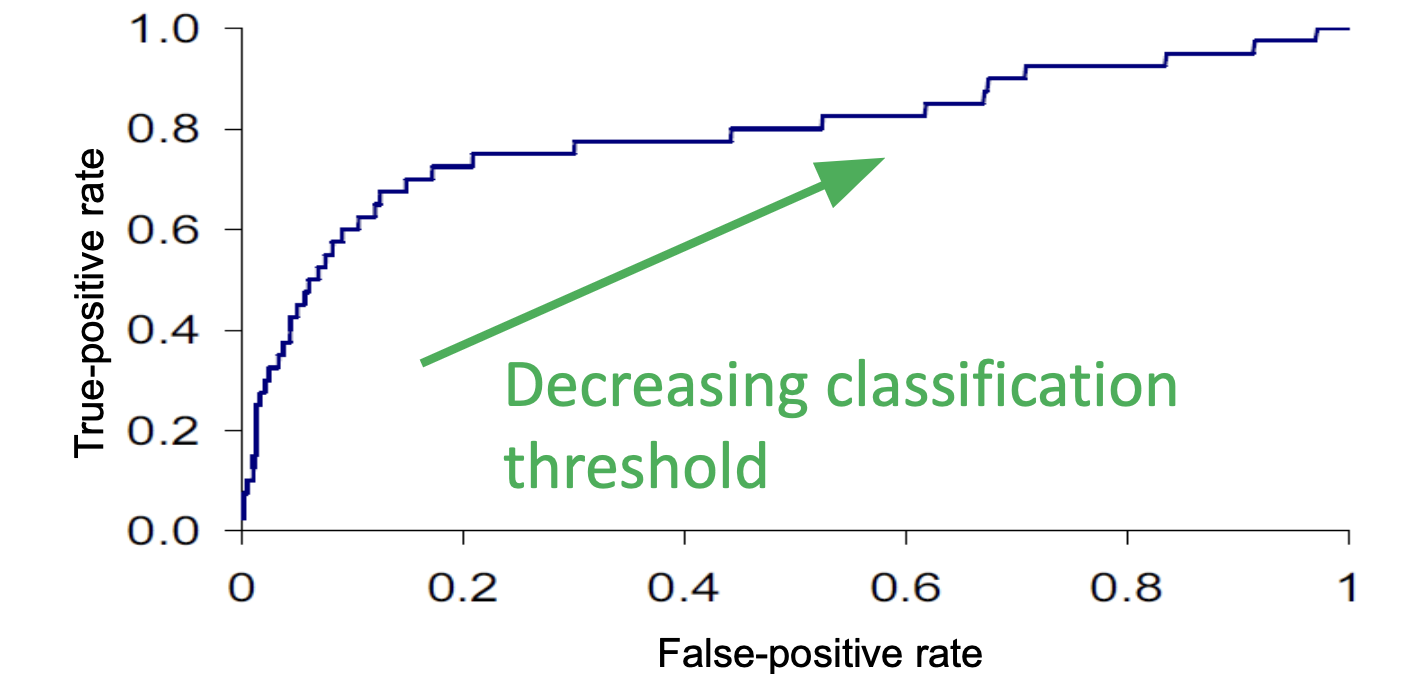
\includegraphics[width=0.7\textwidth]{roc}
    \label{fig:LABEL}
\end{figure}

ROC AUC is the "area under the curse"- a single number that captures the overall quality of the classifier. IT should be between 0.5 (random classifier) and 1.0 (perfect). 

\subsection*{Bias and variance}

% Quick centered image
\begin{figure}[H]
    \centering
    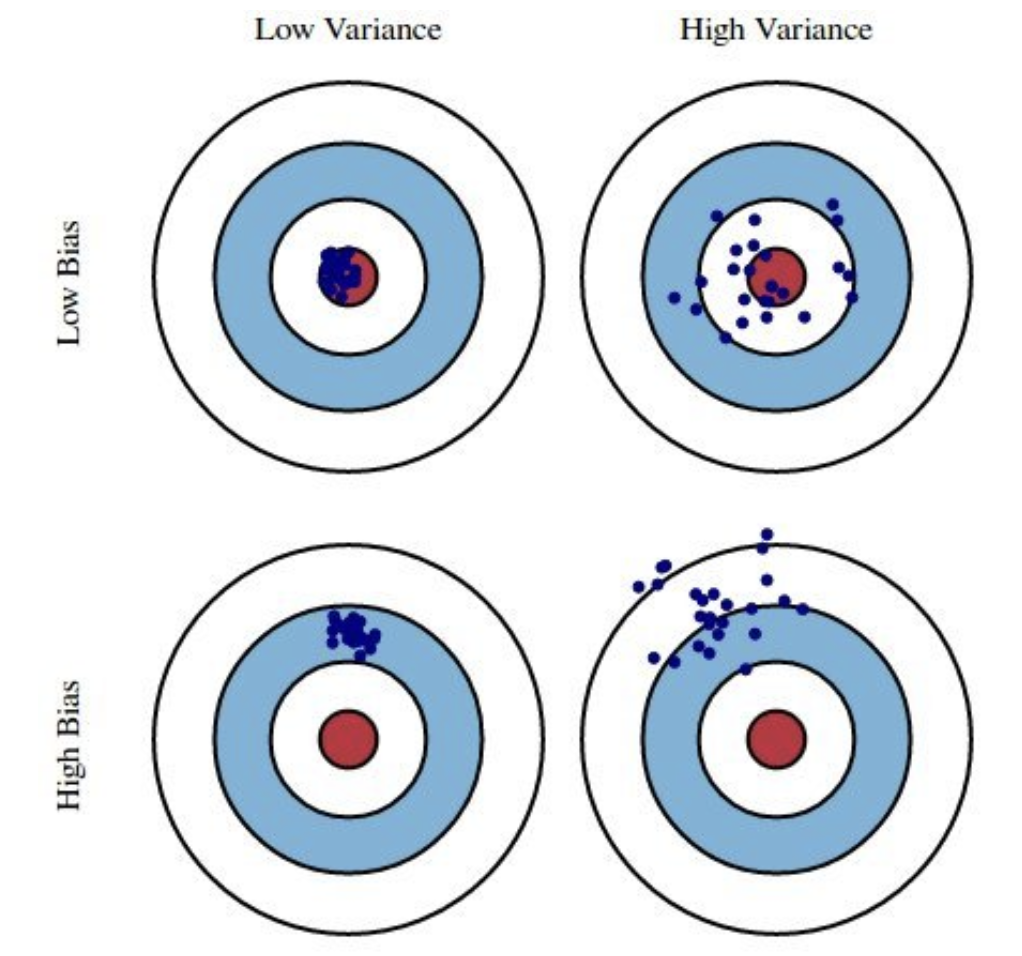
\includegraphics[width=0.5\textwidth]{bias-variance}
    \label{fig:LABEL}
\end{figure}

% Quick centered image
\begin{figure}[H]
    \centering
    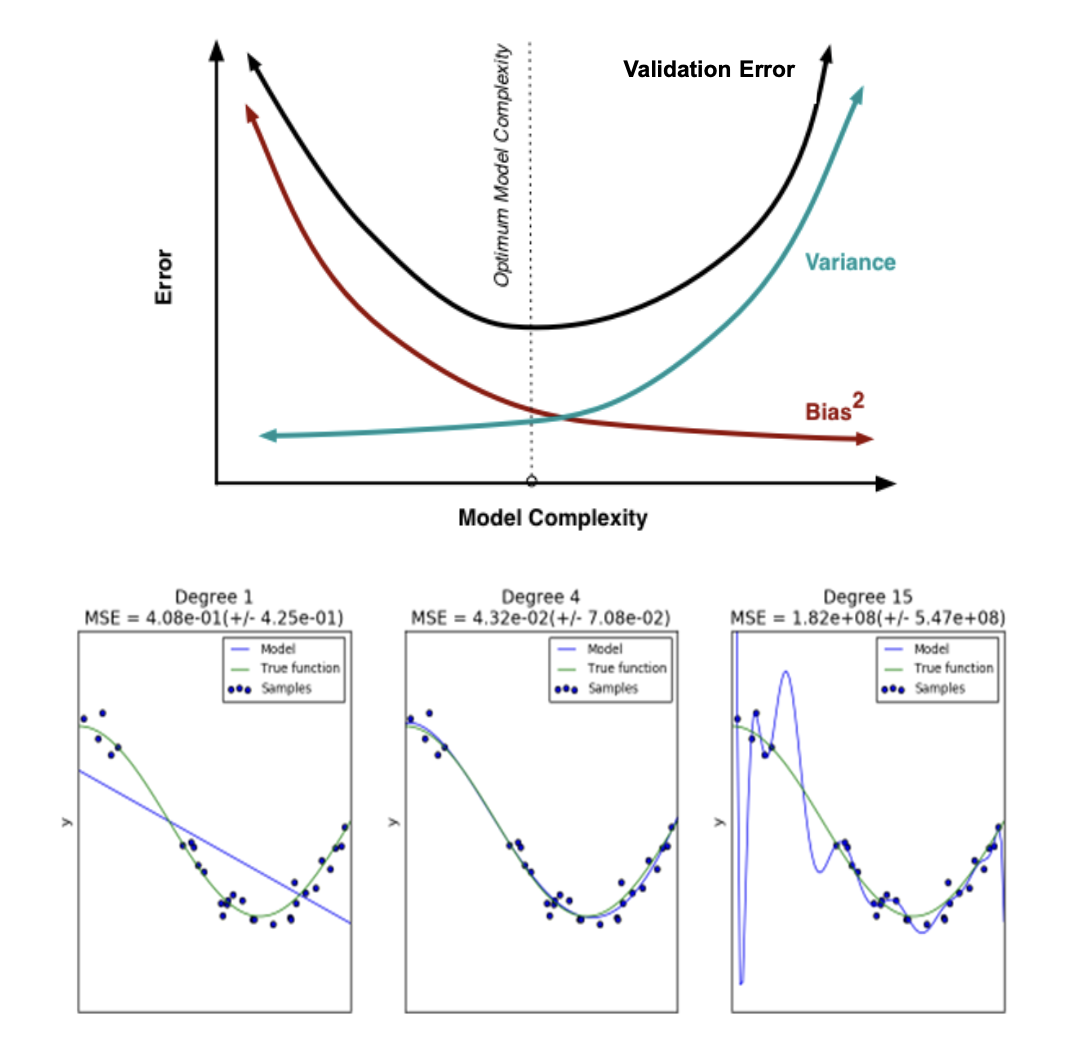
\includegraphics[width=0.7\textwidth]{bias-variance-2}
    \label{fig:LABEL}
\end{figure}

Often we don't have the variance and bias curves... So we use the validation error and training error metrics! 

Thus, bias and variance ban be assessed by comparing the error metric on the training set and the validation set $\Rightarrow$ always \textbf{plot learning curves} (training set size vs. \textcolor{purple}{training}/\textcolor{blue}{validation} errors)

% Quick centered image
\begin{figure}[H]
    \centering
    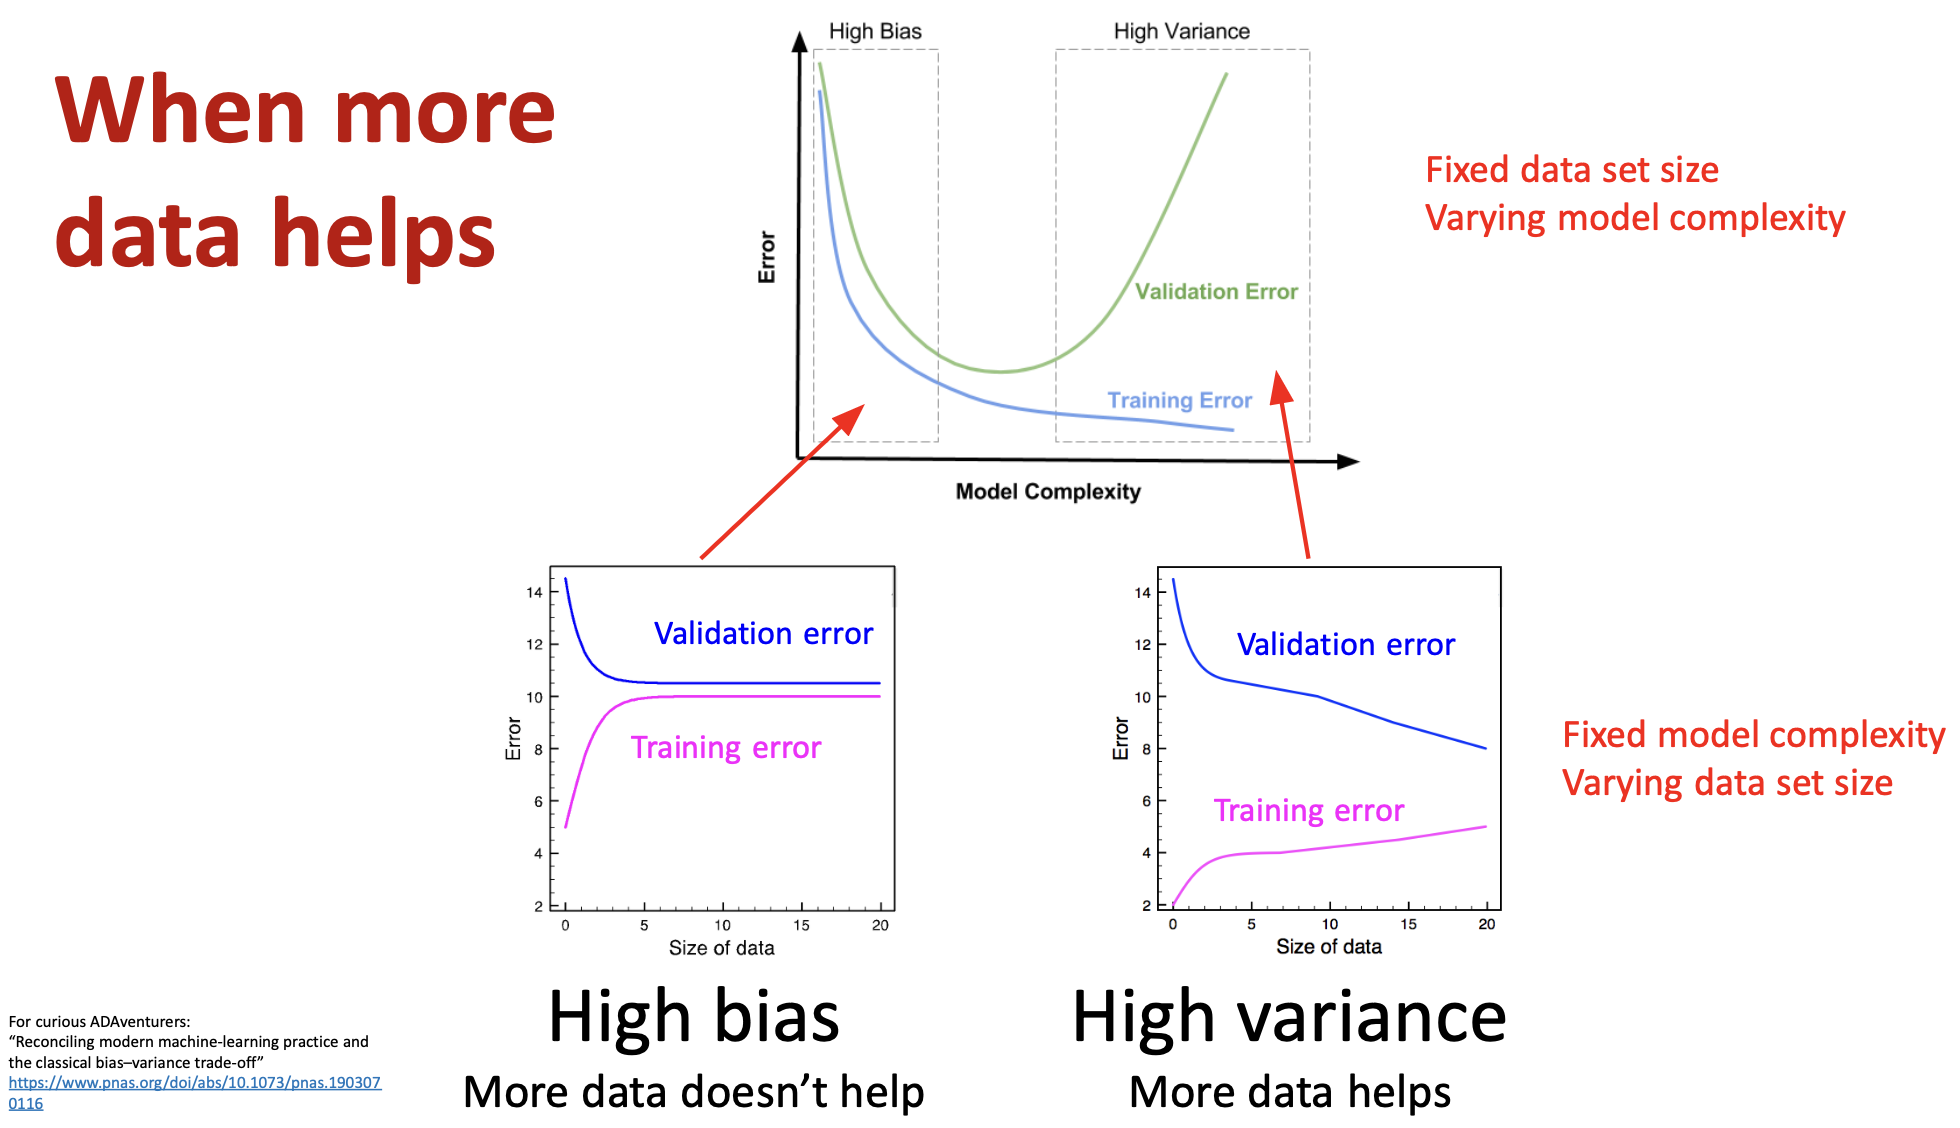
\includegraphics[width=0.8\textwidth]{more-data}
    \label{fig:LABEL}
\end{figure}

\newpage

\section*{Model assessment}

\begin{itemize}
	\item Model assessment is the goal of estimating the performance of a fixed model (i.e, the best model found during model selection)
	\item Ideally under real-world conditions
	\item Use held-out test set that you've never seen during training
\end{itemize}


\end{document}
